% Options for packages loaded elsewhere
\PassOptionsToPackage{unicode}{hyperref}
\PassOptionsToPackage{hyphens}{url}
\PassOptionsToPackage{dvipsnames,svgnames,x11names}{xcolor}
%
\documentclass[
  letterpaper,
  DIV=11,
  numbers=noendperiod,
  oneside]{scrartcl}

\usepackage{amsmath,amssymb}
\usepackage{lmodern}
\usepackage{iftex}
\ifPDFTeX
  \usepackage[T1]{fontenc}
  \usepackage[utf8]{inputenc}
  \usepackage{textcomp} % provide euro and other symbols
\else % if luatex or xetex
  \usepackage{unicode-math}
  \defaultfontfeatures{Scale=MatchLowercase}
  \defaultfontfeatures[\rmfamily]{Ligatures=TeX,Scale=1}
\fi
% Use upquote if available, for straight quotes in verbatim environments
\IfFileExists{upquote.sty}{\usepackage{upquote}}{}
\IfFileExists{microtype.sty}{% use microtype if available
  \usepackage[]{microtype}
  \UseMicrotypeSet[protrusion]{basicmath} % disable protrusion for tt fonts
}{}
\makeatletter
\@ifundefined{KOMAClassName}{% if non-KOMA class
  \IfFileExists{parskip.sty}{%
    \usepackage{parskip}
  }{% else
    \setlength{\parindent}{0pt}
    \setlength{\parskip}{6pt plus 2pt minus 1pt}}
}{% if KOMA class
  \KOMAoptions{parskip=half}}
\makeatother
\usepackage{xcolor}
\usepackage[left=1in,marginparwidth=2.0666666666667in,textwidth=4.1333333333333in,marginparsep=0.3in]{geometry}
\setlength{\emergencystretch}{3em} % prevent overfull lines
\setcounter{secnumdepth}{5}
% Make \paragraph and \subparagraph free-standing
\ifx\paragraph\undefined\else
  \let\oldparagraph\paragraph
  \renewcommand{\paragraph}[1]{\oldparagraph{#1}\mbox{}}
\fi
\ifx\subparagraph\undefined\else
  \let\oldsubparagraph\subparagraph
  \renewcommand{\subparagraph}[1]{\oldsubparagraph{#1}\mbox{}}
\fi

\usepackage{color}
\usepackage{fancyvrb}
\newcommand{\VerbBar}{|}
\newcommand{\VERB}{\Verb[commandchars=\\\{\}]}
\DefineVerbatimEnvironment{Highlighting}{Verbatim}{commandchars=\\\{\}}
% Add ',fontsize=\small' for more characters per line
\usepackage{framed}
\definecolor{shadecolor}{RGB}{241,243,245}
\newenvironment{Shaded}{\begin{snugshade}}{\end{snugshade}}
\newcommand{\AlertTok}[1]{\textcolor[rgb]{0.68,0.00,0.00}{#1}}
\newcommand{\AnnotationTok}[1]{\textcolor[rgb]{0.37,0.37,0.37}{#1}}
\newcommand{\AttributeTok}[1]{\textcolor[rgb]{0.40,0.45,0.13}{#1}}
\newcommand{\BaseNTok}[1]{\textcolor[rgb]{0.68,0.00,0.00}{#1}}
\newcommand{\BuiltInTok}[1]{\textcolor[rgb]{0.00,0.23,0.31}{#1}}
\newcommand{\CharTok}[1]{\textcolor[rgb]{0.13,0.47,0.30}{#1}}
\newcommand{\CommentTok}[1]{\textcolor[rgb]{0.37,0.37,0.37}{#1}}
\newcommand{\CommentVarTok}[1]{\textcolor[rgb]{0.37,0.37,0.37}{\textit{#1}}}
\newcommand{\ConstantTok}[1]{\textcolor[rgb]{0.56,0.35,0.01}{#1}}
\newcommand{\ControlFlowTok}[1]{\textcolor[rgb]{0.00,0.23,0.31}{#1}}
\newcommand{\DataTypeTok}[1]{\textcolor[rgb]{0.68,0.00,0.00}{#1}}
\newcommand{\DecValTok}[1]{\textcolor[rgb]{0.68,0.00,0.00}{#1}}
\newcommand{\DocumentationTok}[1]{\textcolor[rgb]{0.37,0.37,0.37}{\textit{#1}}}
\newcommand{\ErrorTok}[1]{\textcolor[rgb]{0.68,0.00,0.00}{#1}}
\newcommand{\ExtensionTok}[1]{\textcolor[rgb]{0.00,0.23,0.31}{#1}}
\newcommand{\FloatTok}[1]{\textcolor[rgb]{0.68,0.00,0.00}{#1}}
\newcommand{\FunctionTok}[1]{\textcolor[rgb]{0.28,0.35,0.67}{#1}}
\newcommand{\ImportTok}[1]{\textcolor[rgb]{0.00,0.46,0.62}{#1}}
\newcommand{\InformationTok}[1]{\textcolor[rgb]{0.37,0.37,0.37}{#1}}
\newcommand{\KeywordTok}[1]{\textcolor[rgb]{0.00,0.23,0.31}{#1}}
\newcommand{\NormalTok}[1]{\textcolor[rgb]{0.00,0.23,0.31}{#1}}
\newcommand{\OperatorTok}[1]{\textcolor[rgb]{0.37,0.37,0.37}{#1}}
\newcommand{\OtherTok}[1]{\textcolor[rgb]{0.00,0.23,0.31}{#1}}
\newcommand{\PreprocessorTok}[1]{\textcolor[rgb]{0.68,0.00,0.00}{#1}}
\newcommand{\RegionMarkerTok}[1]{\textcolor[rgb]{0.00,0.23,0.31}{#1}}
\newcommand{\SpecialCharTok}[1]{\textcolor[rgb]{0.37,0.37,0.37}{#1}}
\newcommand{\SpecialStringTok}[1]{\textcolor[rgb]{0.13,0.47,0.30}{#1}}
\newcommand{\StringTok}[1]{\textcolor[rgb]{0.13,0.47,0.30}{#1}}
\newcommand{\VariableTok}[1]{\textcolor[rgb]{0.07,0.07,0.07}{#1}}
\newcommand{\VerbatimStringTok}[1]{\textcolor[rgb]{0.13,0.47,0.30}{#1}}
\newcommand{\WarningTok}[1]{\textcolor[rgb]{0.37,0.37,0.37}{\textit{#1}}}

\providecommand{\tightlist}{%
  \setlength{\itemsep}{0pt}\setlength{\parskip}{0pt}}\usepackage{longtable,booktabs,array}
\usepackage{calc} % for calculating minipage widths
% Correct order of tables after \paragraph or \subparagraph
\usepackage{etoolbox}
\makeatletter
\patchcmd\longtable{\par}{\if@noskipsec\mbox{}\fi\par}{}{}
\makeatother
% Allow footnotes in longtable head/foot
\IfFileExists{footnotehyper.sty}{\usepackage{footnotehyper}}{\usepackage{footnote}}
\makesavenoteenv{longtable}
\usepackage{graphicx}
\makeatletter
\def\maxwidth{\ifdim\Gin@nat@width>\linewidth\linewidth\else\Gin@nat@width\fi}
\def\maxheight{\ifdim\Gin@nat@height>\textheight\textheight\else\Gin@nat@height\fi}
\makeatother
% Scale images if necessary, so that they will not overflow the page
% margins by default, and it is still possible to overwrite the defaults
% using explicit options in \includegraphics[width, height, ...]{}
\setkeys{Gin}{width=\maxwidth,height=\maxheight,keepaspectratio}
% Set default figure placement to htbp
\makeatletter
\def\fps@figure{htbp}
\makeatother

\KOMAoption{captions}{tableheading}
\makeatletter
\makeatother
\makeatletter
\makeatother
\makeatletter
\@ifpackageloaded{caption}{}{\usepackage{caption}}
\AtBeginDocument{%
\ifdefined\contentsname
  \renewcommand*\contentsname{Table of contents}
\else
  \newcommand\contentsname{Table of contents}
\fi
\ifdefined\listfigurename
  \renewcommand*\listfigurename{List of Figures}
\else
  \newcommand\listfigurename{List of Figures}
\fi
\ifdefined\listtablename
  \renewcommand*\listtablename{List of Tables}
\else
  \newcommand\listtablename{List of Tables}
\fi
\ifdefined\figurename
  \renewcommand*\figurename{Figure}
\else
  \newcommand\figurename{Figure}
\fi
\ifdefined\tablename
  \renewcommand*\tablename{Table}
\else
  \newcommand\tablename{Table}
\fi
}
\@ifpackageloaded{float}{}{\usepackage{float}}
\floatstyle{ruled}
\@ifundefined{c@chapter}{\newfloat{codelisting}{h}{lop}}{\newfloat{codelisting}{h}{lop}[chapter]}
\floatname{codelisting}{Listing}
\newcommand*\listoflistings{\listof{codelisting}{List of Listings}}
\makeatother
\makeatletter
\@ifpackageloaded{caption}{}{\usepackage{caption}}
\@ifpackageloaded{subcaption}{}{\usepackage{subcaption}}
\makeatother
\makeatletter
\@ifpackageloaded{tcolorbox}{}{\usepackage[many]{tcolorbox}}
\makeatother
\makeatletter
\@ifundefined{shadecolor}{\definecolor{shadecolor}{rgb}{.97, .97, .97}}
\makeatother
\makeatletter
\@ifpackageloaded{sidenotes}{}{\usepackage{sidenotes}}
\@ifpackageloaded{marginnote}{}{\usepackage{marginnote}}
\makeatother
\makeatletter
\makeatother
\ifLuaTeX
  \usepackage{selnolig}  % disable illegal ligatures
\fi
\IfFileExists{bookmark.sty}{\usepackage{bookmark}}{\usepackage{hyperref}}
\IfFileExists{xurl.sty}{\usepackage{xurl}}{} % add URL line breaks if available
\urlstyle{same} % disable monospaced font for URLs
\hypersetup{
  pdftitle={A simple process to get your Shiny app online (securely).},
  pdfauthor={Ronald (Ryy) Glenn Thomas},
  colorlinks=true,
  linkcolor={blue},
  filecolor={Maroon},
  citecolor={Blue},
  urlcolor={Blue},
  pdfcreator={LaTeX via pandoc}}

\title{A simple process to get your Shiny app online (securely).}
\author{Ronald (Ryy) Glenn Thomas}
\date{5/26/23}

\begin{document}
\maketitle
\ifdefined\Shaded\renewenvironment{Shaded}{\begin{tcolorbox}[enhanced, interior hidden, borderline west={3pt}{0pt}{shadecolor}, sharp corners, breakable, frame hidden, boxrule=0pt]}{\end{tcolorbox}}\fi

\renewcommand*\contentsname{Table of contents}
{
\hypersetup{linkcolor=}
\setcounter{tocdepth}{3}
\tableofcontents
}
\marginnote{\begin{footnotesize}

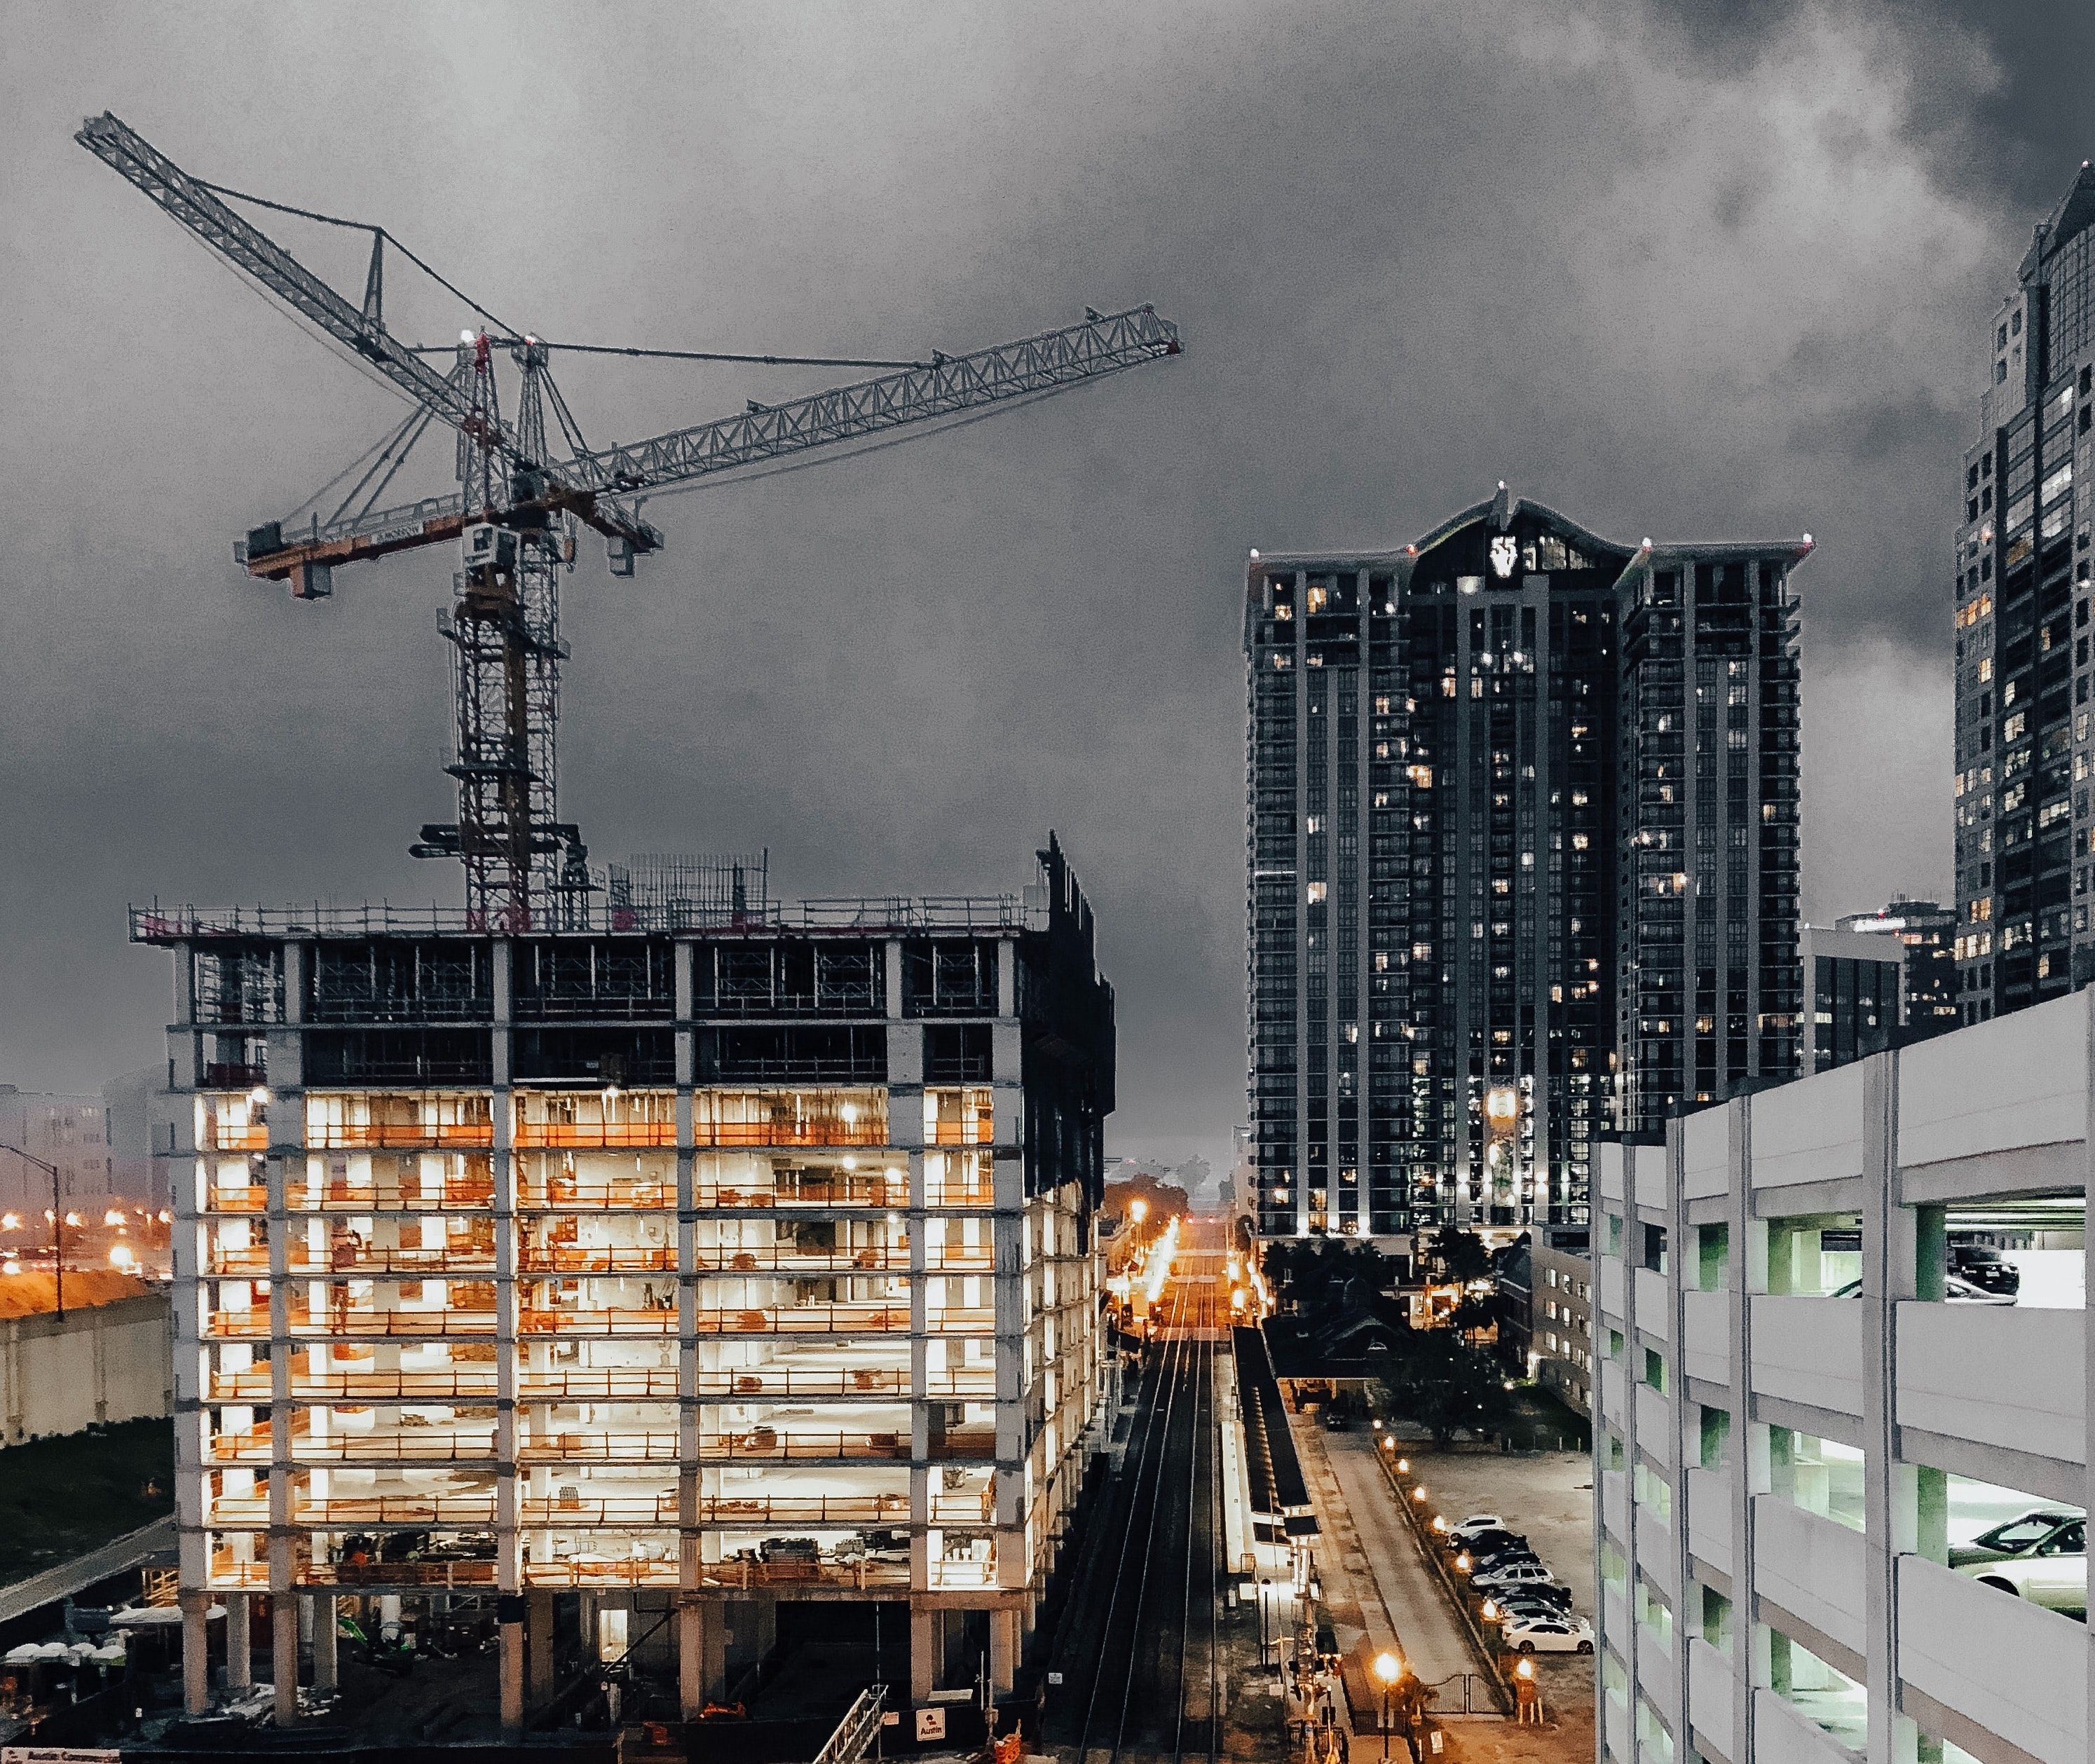
\includegraphics{img/crane.jpg} Photo by Nathan Waters on Unsplash

\end{footnotesize}}

\hypertarget{introduction}{%
\section{Introduction}\label{introduction}}

This is another in a series of posts straightforward, open-source
strategies effectively communicate data analysis results to clients and
collaborators.

In this post we propose a simple method to migrate a shiny app from your
local workstation to the web.

The list of open-source technologies (software stack) we suggest for
employment is: linux, R, Shiny, Docker, and Caddy. In this post we'll
make use of the AWS cloud service. In future posts we'll describe
alternate constructions, e.g.~using the low cost cloud service: Hetzner.

In the following we'll provide a proof-of-concept example of how to
apply these technologies for securely hosting an interactive Shiny
application on the web.

We start with a very simple, but hopefully still useful, stand-alone
Shiny app developed on our local workstation. After some interfacing
with the Amazon web service environment, we'll push the Shiny app into
the cloud, configure a web server, and end up with a secure (encrypted
and authenticated) app running on a website with a custom domain name.

\hypertarget{methods}{%
\section{Methods}\label{methods}}

To begin, lets assume we're just finished developing a new Shiny app,
named \texttt{power1\_shiny}. We have a working directory named
\texttt{power1\_app}. Inside that directory \texttt{power1\_shiny} is a
sub-directory containing the shiny program file \texttt{app.R}.

The methods described here apply generically to any Shiny app, but we'll
use one of our own for illustration). See the \texttt{R/Shiny} code for
our \texttt{power1\_shiny} app (\texttt{app.R}) below.

Our shiny app is designed to be a balance of simple and functional, it
calculates the power for a 2-sample t-test as a function of the
standardized effect size. The app is intentionally minimal; using only
base R functions, with a minimum of reactive widgets and layout
commands.

\begin{Shaded}
\begin{Highlighting}[]
\NormalTok{ui }\OtherTok{\textless{}{-}} \FunctionTok{fluidPage}\NormalTok{(}
\FunctionTok{titlePanel}\NormalTok{(}\StringTok{"Power Calculator for Two Group Parallel Designs"}\NormalTok{),}
\FunctionTok{sliderInput}\NormalTok{(}\StringTok{"N"}\NormalTok{, }\StringTok{"Total Sample Size:"}\NormalTok{, }\AttributeTok{min =} \DecValTok{0}\NormalTok{, }\AttributeTok{max =} \DecValTok{300}\NormalTok{, }\AttributeTok{value =} \DecValTok{100}\NormalTok{),}
\FunctionTok{plotOutput}\NormalTok{(}\StringTok{"plot"}\NormalTok{),}
\FunctionTok{verbatimTextOutput}\NormalTok{(}\StringTok{"eff"}\NormalTok{))}

\NormalTok{server }\OtherTok{\textless{}{-}} \ControlFlowTok{function}\NormalTok{(input, output, session) \{}
\NormalTok{  delta }\OtherTok{=} \FunctionTok{seq}\NormalTok{(}\DecValTok{0}\NormalTok{, }\FloatTok{1.5}\NormalTok{,.}\DecValTok{05}\NormalTok{)}
\NormalTok{  pow }\OtherTok{=} \FunctionTok{reactive}\NormalTok{(}\FunctionTok{sapply}\NormalTok{(delta, }\ControlFlowTok{function}\NormalTok{(x) }\FunctionTok{power.t.test}\NormalTok{(input}\SpecialCharTok{$}\NormalTok{N, }\AttributeTok{d=}\NormalTok{x)}\SpecialCharTok{$}\NormalTok{power ))}
\NormalTok{  eff }\OtherTok{=}  \FunctionTok{renderText}\NormalTok{(}\FunctionTok{power.t.test}\NormalTok{(input}\SpecialCharTok{$}\NormalTok{N, }\AttributeTok{power=}\NormalTok{.}\DecValTok{8}\NormalTok{)}\SpecialCharTok{$}\NormalTok{d)}
\NormalTok{  output}\SpecialCharTok{$}\NormalTok{plot }\OtherTok{\textless{}{-}} \FunctionTok{renderPlot}\NormalTok{(\{}
  \FunctionTok{plot}\NormalTok{(delta, }\FunctionTok{pow}\NormalTok{(), }\AttributeTok{cex=}\FloatTok{1.5}\NormalTok{, }\AttributeTok{ylab=}\StringTok{"power"}\NormalTok{)}
  \FunctionTok{abline}\NormalTok{(}\AttributeTok{h =}\NormalTok{ .}\DecValTok{8}\NormalTok{,  }\AttributeTok{col =} \StringTok{"red"}\NormalTok{, }\AttributeTok{lwd =}\FloatTok{2.5}\NormalTok{, }\AttributeTok{lty =} \DecValTok{4}\NormalTok{)}
  \FunctionTok{abline}\NormalTok{(}\AttributeTok{v =} \FunctionTok{eff}\NormalTok{(), }\AttributeTok{col =} \StringTok{"blue"}\NormalTok{,}\AttributeTok{lwd =}\FloatTok{2.5}\NormalTok{, }\AttributeTok{lty =} \DecValTok{4}\NormalTok{)\})  }
\NormalTok{  output}\SpecialCharTok{$}\NormalTok{eff }\OtherTok{\textless{}{-}} \FunctionTok{renderText}\NormalTok{(}
    \FunctionTok{paste0}\NormalTok{(}\StringTok{"Std. effect detectable with power 80\% = "}\NormalTok{, }\FunctionTok{eff}\NormalTok{()) )}
\NormalTok{\}}
\FunctionTok{shinyApp}\NormalTok{(ui, server)}
\end{Highlighting}
\end{Shaded}

We can test the app locally on our workstation by runnning it with the
following command issued from the \texttt{power1\_app} directory shell
prompt

\begin{Shaded}
\begin{Highlighting}[]
\FunctionTok{zsh}\OperatorTok{\textgreater{}}\NormalTok{ R }\AttributeTok{{-}e} \StringTok{"library(shiny); runApp(\textquotesingle{}power1\_shiny/app.R\textquotesingle{}, launch=T)"}
\end{Highlighting}
\end{Shaded}

This will, in sequence, start the R program, load the Shiny package, run
and launch the app in your default browser.

The margin Figure shows our Shiny app running locally in a browser on
our desktop, it consists of a widget to select the sample size and a
plot to provide a dynamic visualization of the power as a function of
the standardized effect size.

\begin{marginfigure}

{\centering 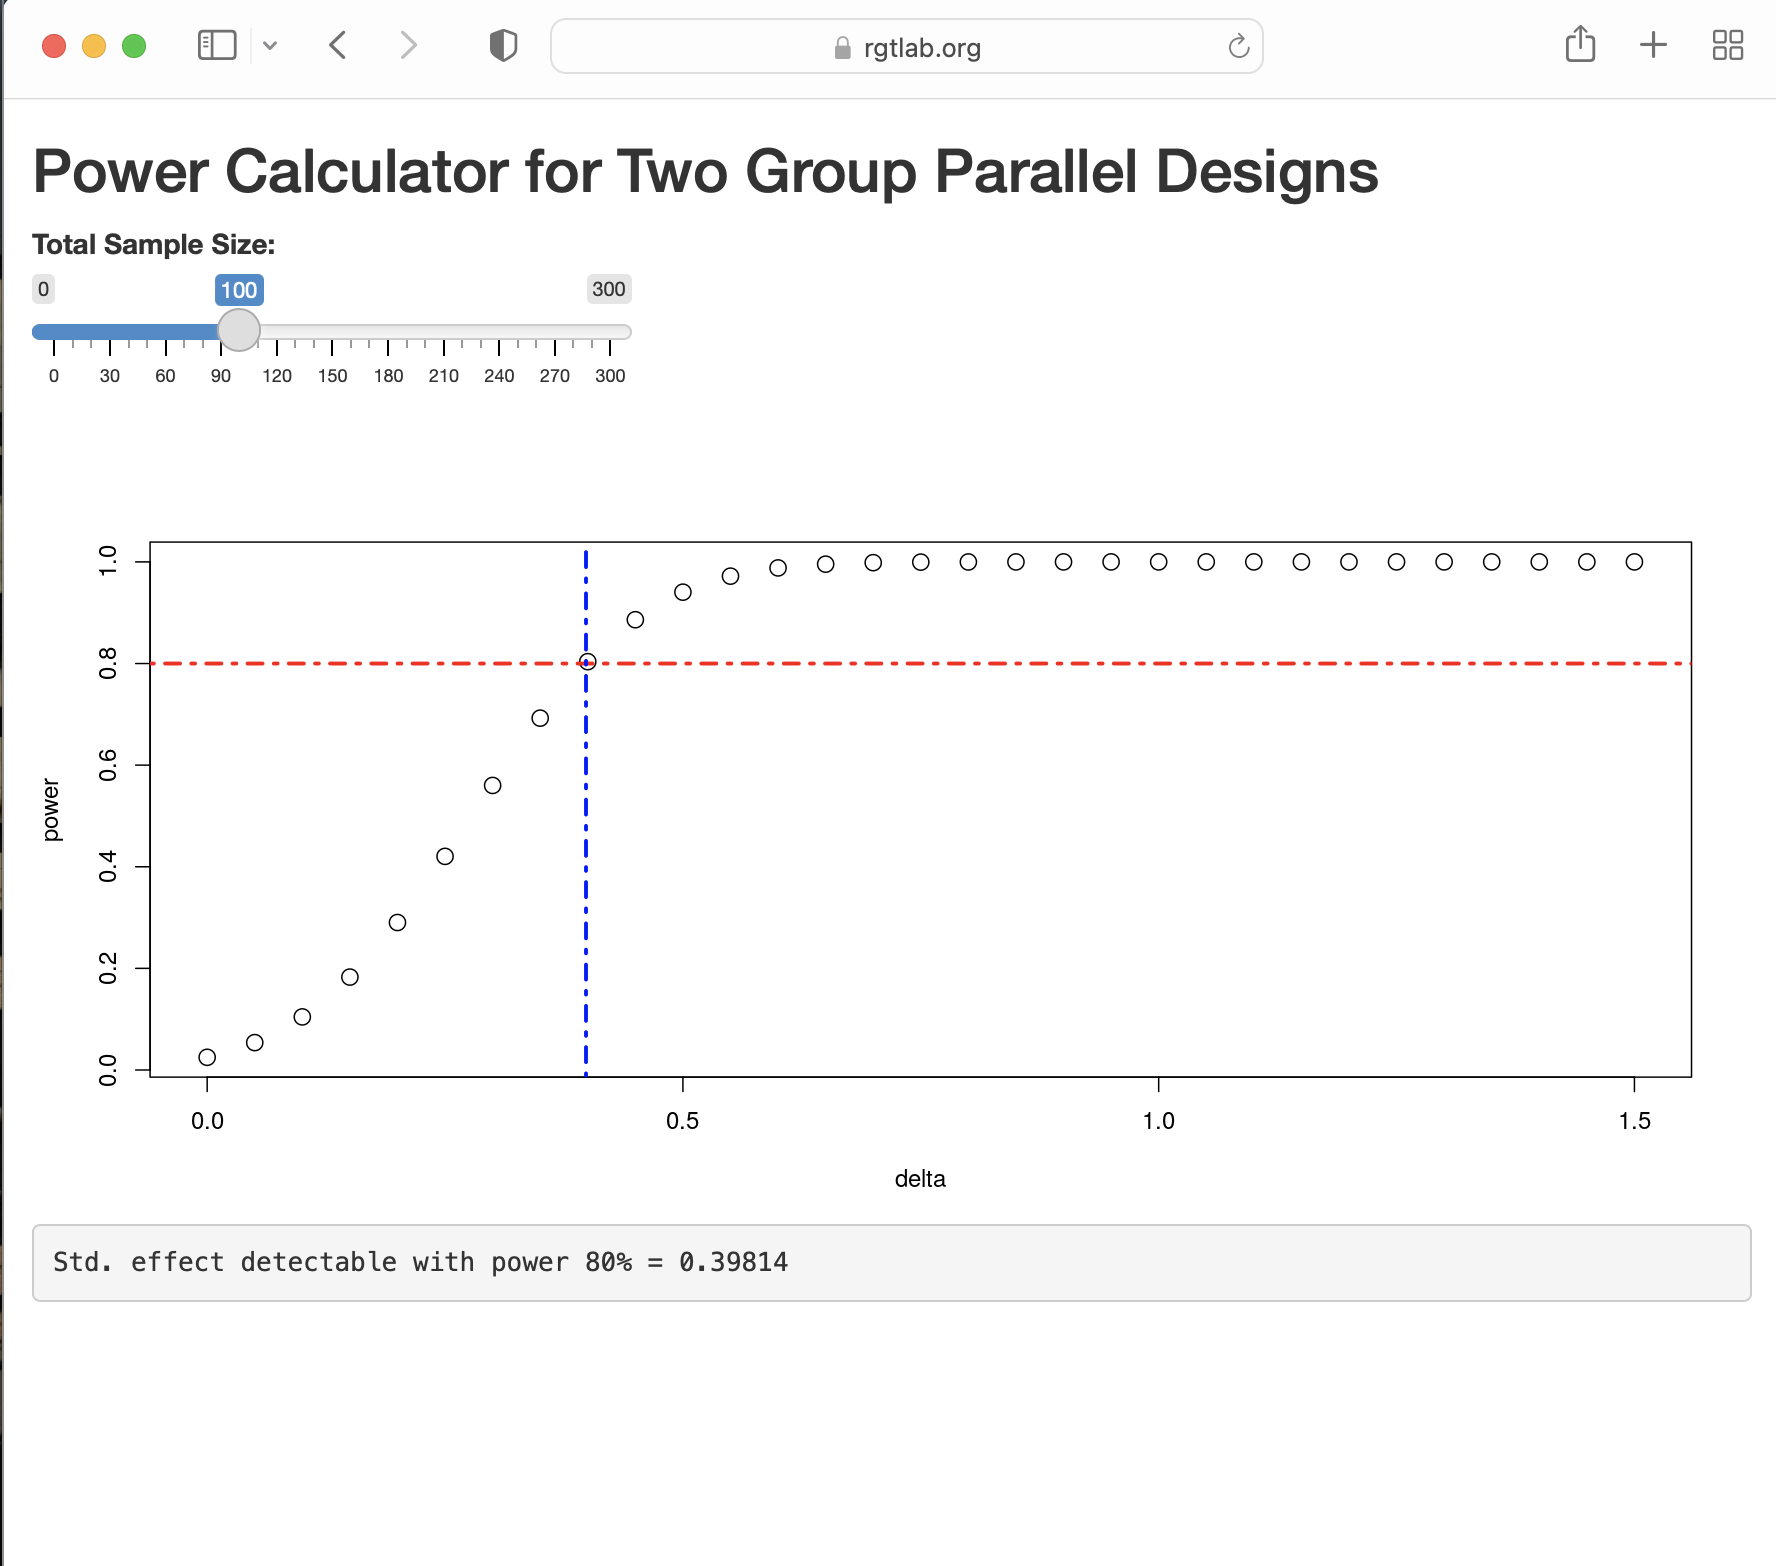
\includegraphics{img/shinyapppower1.png}

}

\caption{\emph{Shiny app}}

\end{marginfigure}

Once we determine our app is working as designed, we move on to the task
of hosting the app on a (virtual) server with the goal of sharing with
our collaborators. There are many ways to accomplish this. Here we'll
describe how to `spin up' a server on Amazon Web Service EC2 and in just
a few steps, through the application of Docker, R, Shiny, and Caddy have
a secure web app running.

\hypertarget{hosting}{%
\section{Hosting}\label{hosting}}

In order to host \texttt{power1\_shiny} online we'll need to complete
the following tasks:

\begin{enumerate}
\def\labelenumi{\arabic{enumi}.}
\tightlist
\item
  create a virtual server with a firewall
\item
  obtain a static IP address
\item
  obtain a domain name
\item
  install and configure a webserver
\item
  obtain and install an SSL certificate
\item
  setup an authentication method and
\item
  configure a reverse proxy method to translate https (port 443)
  requests to Shiny (port 3838).
\end{enumerate}

At first glance these 7 requirements can appear daunting, but on closer
inspection all can be met with relative ease and minimal cost ( using a
cloud-hosting service, e.g.~Amazon's EC2 or Digital Ocean, and a
``leased'' domain name from, e.g.~GoDaddy, or Amazon's Route 53) or at
no cost if you have your own server with IP address, and domain name.

\hypertarget{select-a-hosting-service}{%
\subsection{Select a hosting service}\label{select-a-hosting-service}}

There are a number of cloud based server options: Microsoft Azure,
Oracle, Google Cloud, Amazon AWS EC2, Digital Ocean to name a few. Each
has their own approach to setting up a custom virtual server. Several
have free or low-cost service tiers available.

An overview of the process with EC2 follows. (Detailed instructions for
AWS EC2 were described in an earlier post:
\url{https://focusonr.org/posts/setupaws/})

step 0. Create an AWS account or sign in and navigate to the EC2
dashboard. step 1. Set up an working environment with AWS server. a.
define secure shell (ssh) key-pair b. configure firewall. c.~obtain
static IP. d.~obtain domain name.

\begin{verbatim}
Once the environment is set up
\end{verbatim}

step 2. a. select instance operating system (\texttt{ubuntu}) and type
(\texttt{t2-micro}) b. launch server

Once the server is available connect via ssh.

\begin{Shaded}
\begin{Highlighting}[]
\FunctionTok{ssh} \AttributeTok{{-}i} \StringTok{"\textasciitilde{}/.ssh/power1\_app\_ssh.pem"}\NormalTok{  ubuntu@rgtlab.org}
\end{Highlighting}
\end{Shaded}

or using the \texttt{config} setup described in Tip 1.

\begin{Shaded}
\begin{Highlighting}[]
\FunctionTok{ssh}\NormalTok{ rgtlab.org }
\end{Highlighting}
\end{Shaded}

The only necessary software to install is Docker and Caddy. Install them
with the following commands:

\begin{Shaded}
\begin{Highlighting}[]
\FunctionTok{sudo}\NormalTok{ apt install docker.io}
\FunctionTok{sudo}\NormalTok{ apt install }\AttributeTok{{-}y}\NormalTok{ debian{-}keyring debian{-}archive{-}keyring apt{-}transport{-}https}
\ExtensionTok{curl} \AttributeTok{{-}1sLf} \StringTok{\textquotesingle{}https://dl.cloudsmith.io/public/caddy/stable/gpg.key\textquotesingle{}} \KeywordTok{|} \DataTypeTok{\textbackslash{}}
\FunctionTok{sudo}\NormalTok{ gpg }\AttributeTok{{-}{-}dearmor} \AttributeTok{{-}o}\NormalTok{ /usr/share/keyrings/caddy{-}stable{-}archive{-}keyring.gpg}
\ExtensionTok{curl} \AttributeTok{{-}1sLf} \StringTok{\textquotesingle{}https://dl.cloudsmith.io/public/caddy/stable/debian.deb.txt\textquotesingle{}} \KeywordTok{|} \DataTypeTok{\textbackslash{}}
\FunctionTok{sudo}\NormalTok{ tee /etc/apt/sources.list.d/caddy{-}stable.list}
\FunctionTok{sudo}\NormalTok{ apt update}
\FunctionTok{sudo}\NormalTok{ apt install caddy}
\end{Highlighting}
\end{Shaded}

At this point we have a customized virtual server with a static IP
address, unique domain name and firewall in place. In other words, items
1, 2, and 3 from our `hosting' list above are taken care of.

\hypertarget{website}{%
\subsection{Website}\label{website}}

To configure the web server and containerize our app we need to add
three files to the server, to go along with our Shiny app in the
\texttt{power1\_app} directory and move all files to the server.

The three configuation files are:

\begin{enumerate}
\def\labelenumi{\arabic{enumi}.}
\tightlist
\item
  a Docker configuration file (default name \texttt{Dockerfile})
\end{enumerate}

\marginnote{\begin{footnotesize}

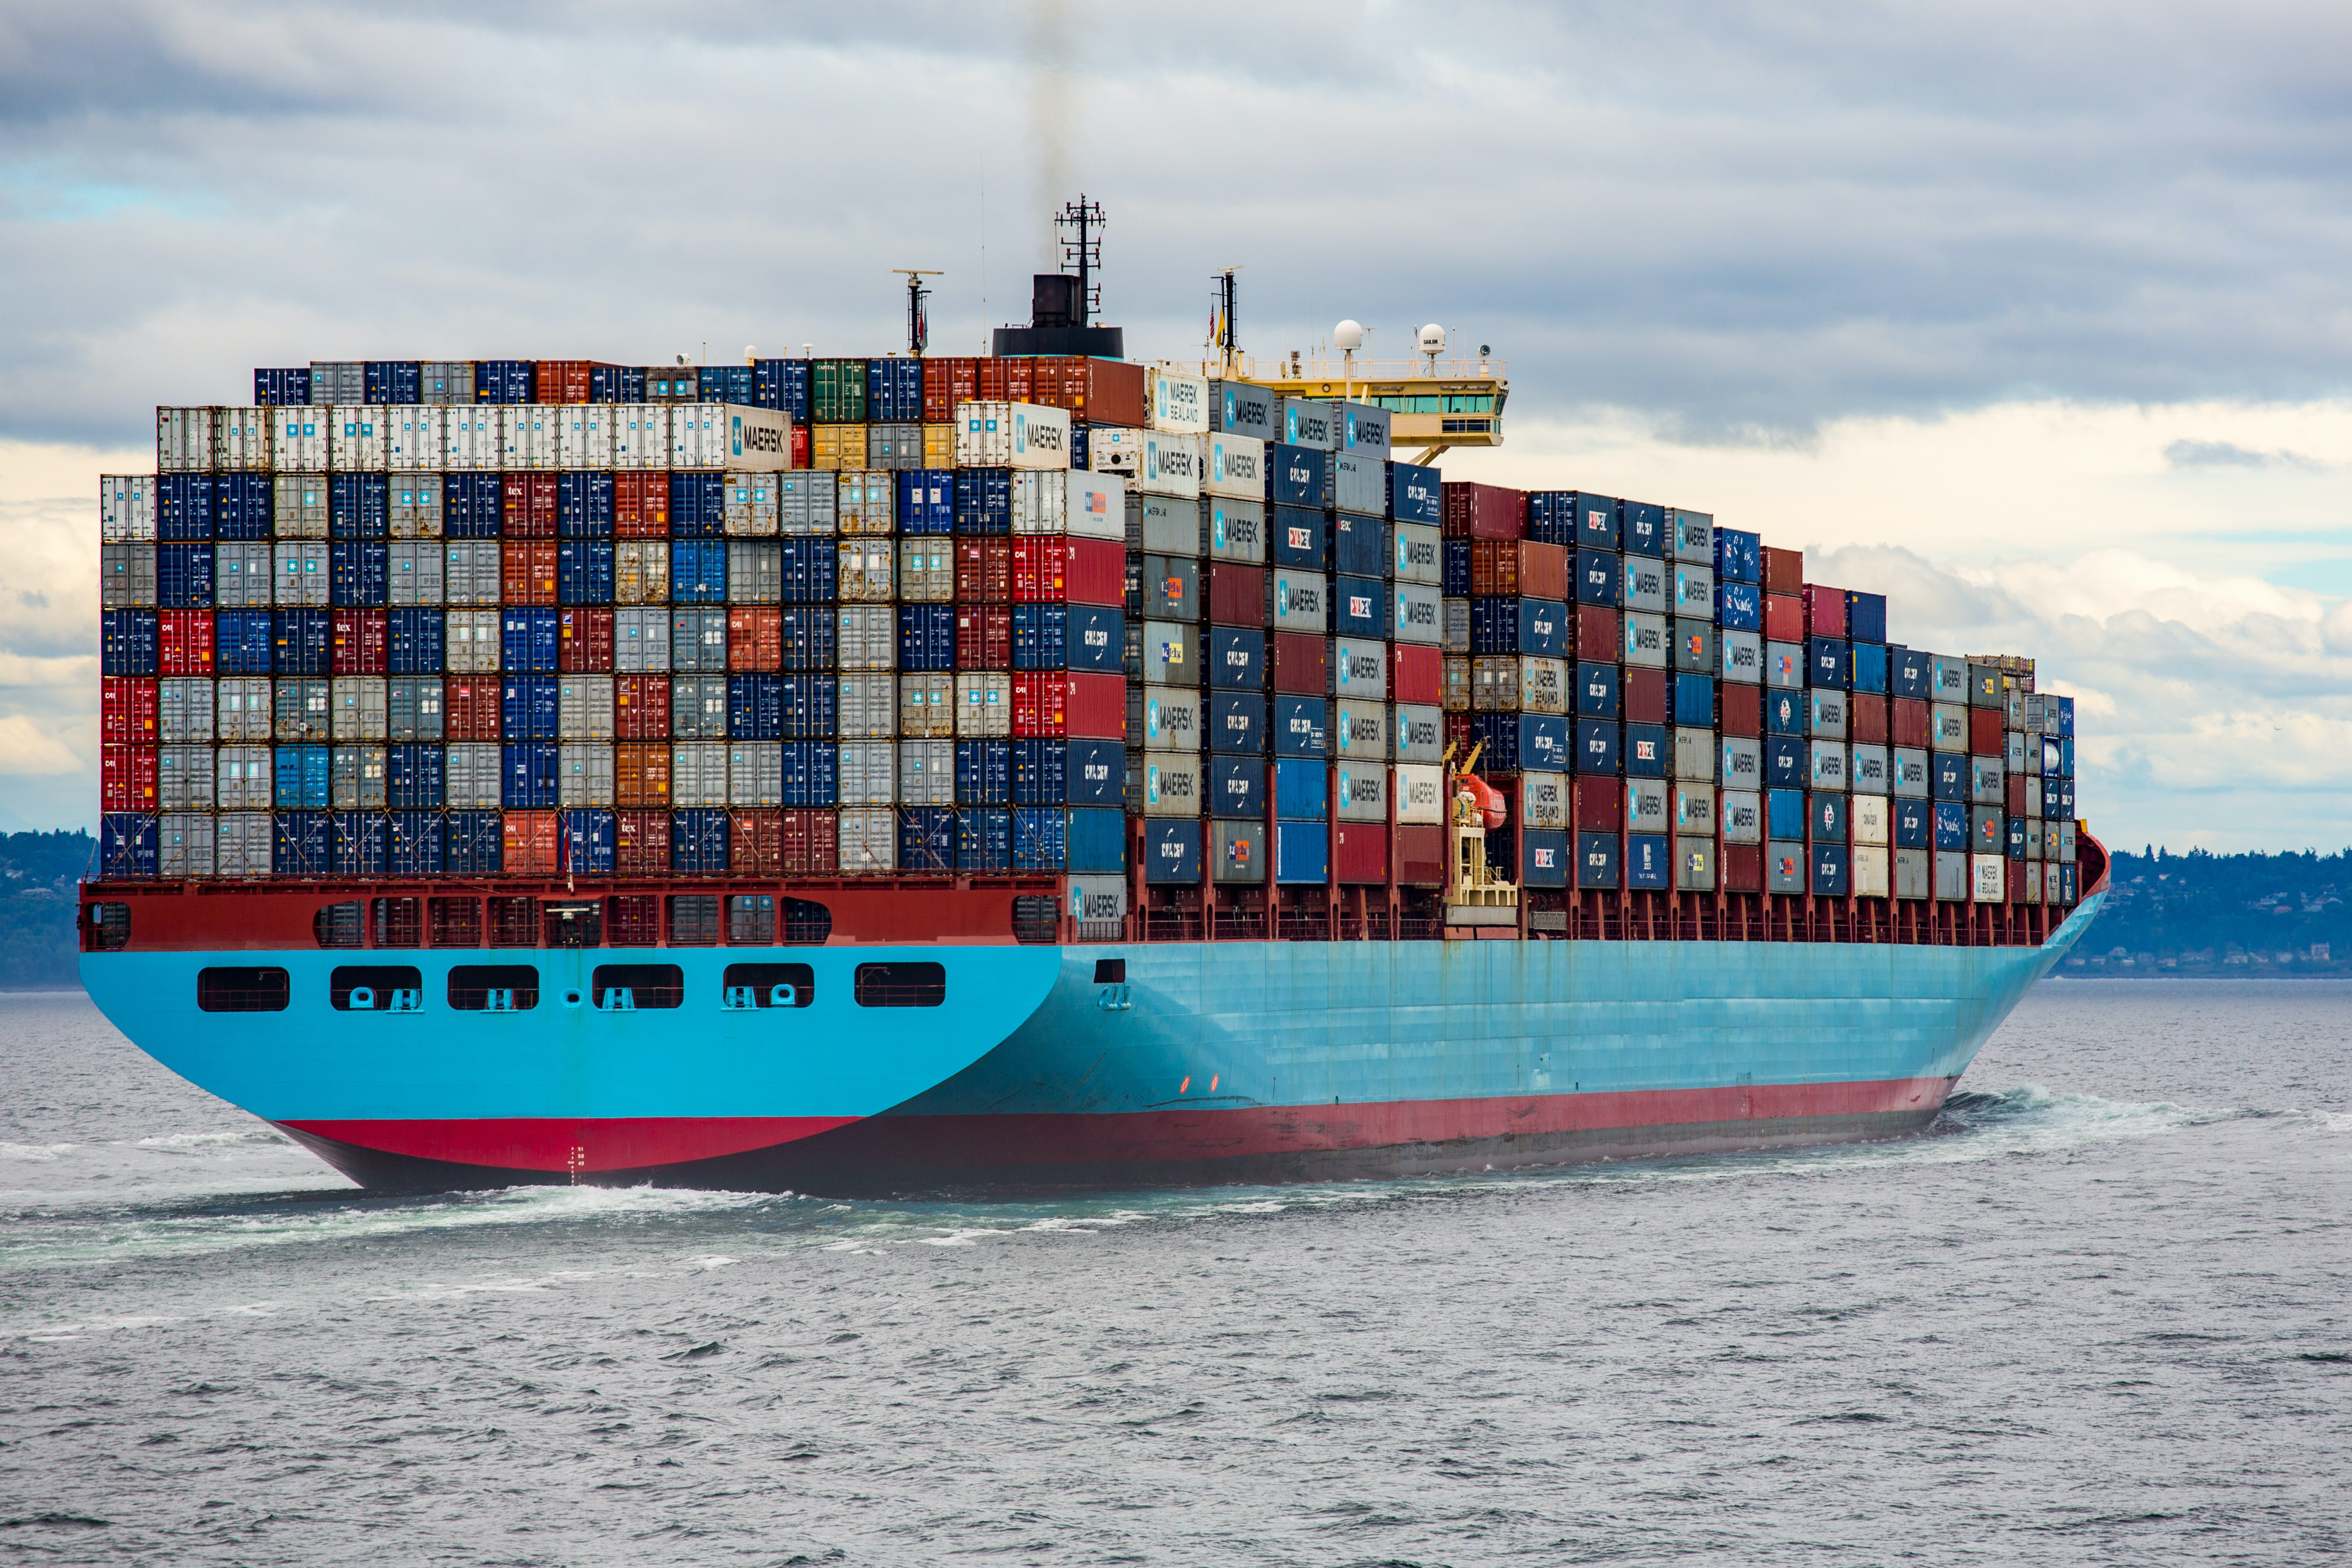
\includegraphics{img/docker1.jpg} Photo by Ian Taylor on Unsplash

\end{footnotesize}}

We'll use docker to access R/Shiny. Here is our minimal dockerfile:

\begin{Shaded}
\begin{Highlighting}[]
\NormalTok{FROM rocker}\SpecialCharTok{/}\NormalTok{shiny}\SpecialCharTok{:}\DecValTok{4}\NormalTok{.}\FloatTok{2.0}
\NormalTok{COPY }\SpecialCharTok{/}\NormalTok{power1\_shiny}\SpecialCharTok{/}\ErrorTok{*} \ErrorTok{/}\NormalTok{srv}\SpecialCharTok{/}\NormalTok{shiny}\SpecialCharTok{{-}}\NormalTok{server}\SpecialCharTok{/}
\NormalTok{CMD [}\StringTok{"/usr/bin/shiny{-}server"}\NormalTok{]}
\end{Highlighting}
\end{Shaded}

This file instructs Docker to build a container based on a Rocker/Shiny
image (which is a ubuntu image with R and Shiny installed) then copy
into the container the \texttt{power1\_shiny} directory containing the
shiny code and finally launch Shiny server listening on (default) port
3838. We placed the \texttt{power1\_shiny/app.R} code in the default
location \texttt{/srv/shiny-server} so we only need to start the server
and it will find the shiny program.

\begin{enumerate}
\def\labelenumi{\arabic{enumi}.}
\setcounter{enumi}{1}
\tightlist
\item
  a Caddy web server configuration file (default name
  \texttt{Caddyfile})
\end{enumerate}

We'll use \texttt{Caddy} as our web server. Caddy is an open-source tool
that has the very useful feature of automating the acquiring and
installing of an SSL certificate. (An SSL cert is required by most
browsers to use the encrypted communication protocol \texttt{https}.)

Caddy is configured with a file named \texttt{Caddyfile}. We use the
caddy configuration file to specify three critical things.

\begin{enumerate}
\def\labelenumi{\arabic{enumi}.}
\tightlist
\item
  the site domain name.
\item
  the authentication pair login/hash-password, for each user and
\item
  the `reverse proxy' map that redirects requests to port 443 (ssl port)
  onto port 3838 (Shiny port) in the docker container.
\end{enumerate}

Our barebones Caddyfile looks like this:

\begin{Shaded}
\begin{Highlighting}[]
\NormalTok{rgtlab.org \{}
\NormalTok{    basicauth }\SpecialCharTok{*} \ErrorTok{/}\NormalTok{power1\_shiny}\SpecialCharTok{/}\ErrorTok{*}\NormalTok{ \{}
\NormalTok{        bob }\SpecialCharTok{$}\NormalTok{2a}\SpecialCharTok{$}\DecValTok{14}\SpecialCharTok{$}\NormalTok{pYWd5O7JqNeGLS4m4CKkzemM2pq5ezn9bcTDowofZTl5wRVl8NTJm}
\NormalTok{    \}}
\NormalTok{    root }\SpecialCharTok{*} \ErrorTok{/}\NormalTok{var}\SpecialCharTok{/}\NormalTok{www}\SpecialCharTok{/}\NormalTok{html}
\NormalTok{    handle\_path }\SpecialCharTok{/}\NormalTok{power1\_shiny}\SpecialCharTok{/}\ErrorTok{*}\NormalTok{ \{}
\NormalTok{            reverse\_proxy }\DecValTok{0}\NormalTok{.}\DecValTok{0}\NormalTok{.}\FloatTok{0.0}\SpecialCharTok{:}\DecValTok{3838}
\NormalTok{    \}}
\NormalTok{    file\_server}
\NormalTok{\}}
\end{Highlighting}
\end{Shaded}

We can accomplish what we need for items 4, 5, 6 and 7 through the
Caddyfile.

Note:

\begin{itemize}
\tightlist
\item
  rgtlab.org is our domain name
\item
  the basicauth directive specifies login credentials for bob (password:
  vanilla47)
\item
  \texttt{handle\_path} maps all https requests to port 3838 where Shiny
  is listening.
\item
  \texttt{root} directive tells Caddy where to look for the
  \texttt{index.html} file.
\end{itemize}

Providing our servers domain name, \texttt{rgtlab.org} is sufficient to
initiate an exchange with the \texttt{letsencrypt} service to generates
an SSL certificate.

And the third file is the \texttt{index.html} file to provide a launch
page for the app.

\begin{Shaded}
\begin{Highlighting}[]
\SpecialCharTok{\textless{}!}\NormalTok{DOCTYPE html}\SpecialCharTok{\textgreater{}}
\ErrorTok{\textless{}}\NormalTok{html}\SpecialCharTok{\textgreater{}}
  \ErrorTok{\textless{}}\NormalTok{body}\SpecialCharTok{\textgreater{}}
    \ErrorTok{\textless{}}\NormalTok{h1}\SpecialCharTok{\textgreater{}}\NormalTok{Power1 app}\SpecialCharTok{\textless{}}\ErrorTok{/}\NormalTok{h1}\SpecialCharTok{\textgreater{}}
    \ErrorTok{\textless{}}\NormalTok{ul}\SpecialCharTok{\textgreater{}}
      \ErrorTok{\textless{}}\NormalTok{li}\SpecialCharTok{\textgreater{}}\ErrorTok{\textless{}}\NormalTok{a href}\OtherTok{=}\StringTok{"./power1\_shiny/"}\SpecialCharTok{\textgreater{}}\NormalTok{Power1 app}\SpecialCharTok{\textless{}}\ErrorTok{/}\NormalTok{a}\SpecialCharTok{\textgreater{}}\ErrorTok{\textless{}/}\NormalTok{li}\SpecialCharTok{\textgreater{}}
    \ErrorTok{\textless{}/}\NormalTok{ul}\SpecialCharTok{\textgreater{}}
  \ErrorTok{\textless{}/}\NormalTok{body}\SpecialCharTok{\textgreater{}}
\ErrorTok{\textless{}/}\NormalTok{html}\SpecialCharTok{\textgreater{}} 
\end{Highlighting}
\end{Shaded}

Once the three config files and the the Shiny code directory are in
place copy the \texttt{power1\_app} directory to the server
\texttt{rgtlab.org} with the command:

\begin{Shaded}
\begin{Highlighting}[]
\FunctionTok{scp} \AttributeTok{{-}i} \StringTok{"\textasciitilde{}/.ssh/power1\_app\_ssh.pem"} \AttributeTok{{-}r}\NormalTok{ \textasciitilde{}/prj/power1\_app/  ubuntu@rgtlab.org:\textasciitilde{}}
\end{Highlighting}
\end{Shaded}

Lastly, ssh to the server and cd to \texttt{power1\_app} directory

copy \texttt{Caddyfile} to location caddy expects in \texttt{/etc/caddy}
directory

\begin{Shaded}
\begin{Highlighting}[]
\FunctionTok{sudo}\NormalTok{ cp ./Caddyfile /etc/caddy/Caddyfile }
\end{Highlighting}
\end{Shaded}

copy \texttt{index.html} to location caddy expects in
\texttt{/var/www/html} directory

\begin{Shaded}
\begin{Highlighting}[]
\FunctionTok{cp}\NormalTok{  ./index.html /var/www/html/index.html }
\end{Highlighting}
\end{Shaded}

and run the following command to

build the Docker container on \texttt{rgtlab.org}

\begin{Shaded}
\begin{Highlighting}[]
\ExtensionTok{docker}\NormalTok{ build }\AttributeTok{{-}t}\NormalTok{ power1\_image .}
\end{Highlighting}
\end{Shaded}

create container and run

\begin{Shaded}
\begin{Highlighting}[]
\ExtensionTok{docker}\NormalTok{ run }\AttributeTok{{-}d} \AttributeTok{{-}{-}name}\OperatorTok{=}\NormalTok{power1\_shiny }\AttributeTok{{-}p}\NormalTok{ 3838:3838 }\AttributeTok{{-}{-}restart}\OperatorTok{=}\NormalTok{always power1\_image}
\end{Highlighting}
\end{Shaded}

restart Caddy

\begin{Shaded}
\begin{Highlighting}[]
\FunctionTok{sudo}\NormalTok{ systemctl reload caddy}
\end{Highlighting}
\end{Shaded}

App launch page is now available at \texttt{https://rgtlab.org}.

and you're good to go!

\hypertarget{tip-construct-ssh-config-file.}{%
\subsection{Tip construct ssh config
file.}\label{tip-construct-ssh-config-file.}}

For convenience, construct a \texttt{config} file in
\texttt{\textasciitilde{}/.ssh} as:

\begin{Shaded}
\begin{Highlighting}[]
\ExtensionTok{Host}\NormalTok{ rgtlab.org}
\ExtensionTok{HostName}\NormalTok{ 13.57.139.31 }\CommentTok{\# static IP}
\ExtensionTok{StrictHostKeyChecking}\NormalTok{ no  }\CommentTok{\#avoid known host file error message}
\ExtensionTok{User}\NormalTok{ ubuntu }\CommentTok{\# default user on ubuntu server}
\ExtensionTok{Port}\NormalTok{ 22  }\CommentTok{\# the default port ssh uses}
\ExtensionTok{IdentityFile}\NormalTok{ \textasciitilde{}/.ssh/power1\_app.pem}
\end{Highlighting}
\end{Shaded}

then you can ssh into the new server with

\begin{Shaded}
\begin{Highlighting}[]
\FunctionTok{sh}\OperatorTok{\textgreater{}}\NormalTok{ ssh rgtlab.org }
\end{Highlighting}
\end{Shaded}




\end{document}
